\chapter{Quality Control of RPCs}
The Resistive Plate Chamber (RPC) is chosen as the sensitive detector of the ICAL. The ICAL requires approximately 30000 RPCs to function at its full capacity. The INO~Project is proposed to operate at-least for 20 years. All the RPCs thus must operate without showing any sugnificant ageing during the the period of operation. Hence, various tests are performed during and after production of the RPCs.
\begin{figure}[h]
  \centering
  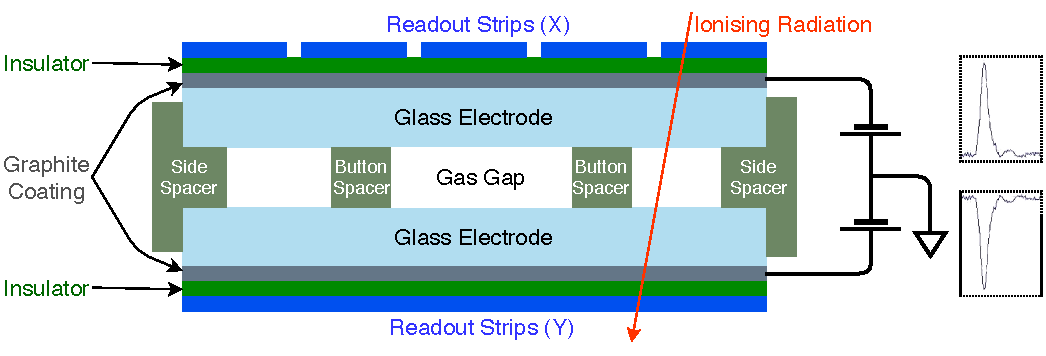
\includegraphics[width=0.6\textwidth]{basic_rpc.pdf}
  \caption{Schematic of a Resistive Plate Chamber.}
  \label{fig:rpc}
\end{figure}

The RPCs going to be used in ICAL is made of glass. The two glass plates, kept at an uniform distance of 2\,mm using the help of poly-carbonate buttons, are sealed from four sides to create a leak-tight gas-gap. Both of the outer sides of the gap are coated with semi-resistive graphite paint to form the electrodes where the high voltages can be applied. A mixture of gas is then flown inside the gap. In the ICAL, the gas mixture is composed of R134a\,(95.2\%), iso-C$_4$H$_{10}$\,(4.5\%) and SF$_6$\,(0.3\%).\footnote{R134a is a commercial name of 1,1,1,2-Tetrafluoroethane.} The R134a acts as the target medium for the incident particles. The electrons emitted in the ionisation process initiated by the passing particles then create avalanche under influence of the applied electric field. The signal of the avalanche is then sensed by two copper pickup panels on the both sides of the gap. The iso-C$_4$H$_{10}$ act as a photon-quencher absorbing the photons emitted in the recombination process limiting the formation of secondary avalanches. On the other hand, the SF$_6$ being an electro-negative gas, acts as an electron-quencher which localises the singnal in a small area yielding better position resolution.

During the up-time of ICAL detector, more than 200000\,litres of the gas mixture will be circulating inside the 30000 RPCs. A closed-loop gas circulating system (CLS) is designed for this purpose whose main aim is to recirculate the gas mixture, minimising the wastage of gas. This pose an additional challenge of keeping the CLS free of contaminations. The leakage of outside atmosphere into the system will introduce water vapour and oxygen inside the RPCs which can increase the risk of damaging the RPCs\cite{rpc_c,rpc_w}. The fuorine present in the RPC gas mixture can produde hydrofluoric after reating with the water vapour during avalanche. The hydrofluoric acid which is corrosive to glass, can ruin the inside surface of the gas gaps. On the other hand, the oxygen being an electro-negative in nature, can affect the performance of the detector. Due to these reasons, a proper leak test is required to be performed on all the glass gaps during the production as~well~as the time of operation. Moreover, the impurities in the CLS also needed to be monitored during the operation of ICAL.

\section{Leak Test of RPCs}
To estimate the leakage, the RPC is first pressurised up-to 45\,mmWC above the atmospheric pressure and then sealed.\footnote{Millimetres water column, abbreviated to mmH$_2$O or mmWC, is a unit of pressure. It is the pressure required to support a water column of the specified height. 1\,mmWC\,$\simeq$\,0.098\,mbar.} The the pressure inside the RPC is monitored over a long period of time. The schematics of a typical leak test setup is shown in Figure~\ref{fig:test_rpc}. 
\begin{figure}
  \centering
  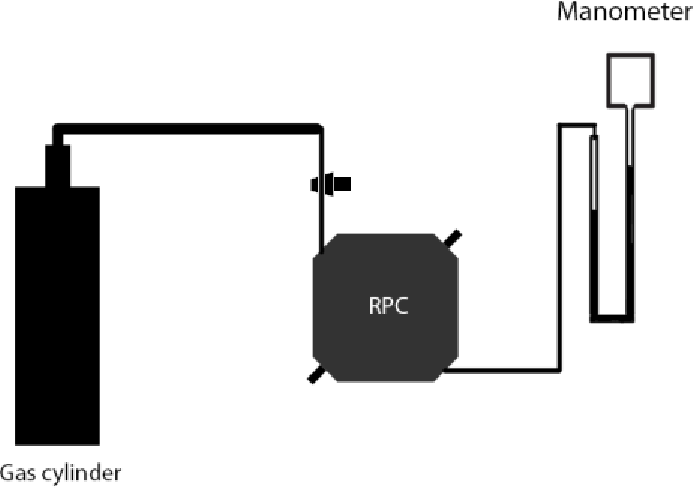
\includegraphics[width=0.6\textwidth]{test_rpc.pdf}
  \caption{Schematics of a typical leak test setup.}
  \label{fig:test_rpc}
\end{figure}
A conventional choice of the sensor to monitor the pressure inside the RPC is the manometer setup as shown in Figure~\ref{fig:test_rpc}. Now, the limitation of leak rate estimation using the manometer comes from its observable quantity. The manometer measures the difference between two pressures $\left(\Delta P\right)$, the atmoshperic pressure $\left(P_{\mathrm{rpc}}\right)$ and the RPC pressure $\left(P_{\mathrm{atm}}\right)$, which can be widely effected by the change of the atmospheric pressure, the room temperature and the volume of the chamber. Hence, the leak estimation using an manometer is only valid in two scenarios, (i) if the atmospheric pressure, the room temperature and the volume of the chamber are kept constant and/or (ii) if the leak rate is very large.

But both the atmospheric pressure and room temperature widely on the ambient pressure and temperature which is constantly affected by the solar atmospheric tides and changes in weather.\footnote{The solar atmospheric tides are generated by the periodic heating of the atmosphere by the Sun. This regular diurnal cycle in heating generates tides in atmosphere that have periods related to the solar day.} In the following, it will be established that the volume of the RPC gaps also changes with the variation of the ambient pressure and temperature. Moreover, if the leak from the RPCs are very small then it nearly impossible to detect.

Hence, a different leak test method along with the test setup is developed to overcome the aforesaid limiatations. The setup and technique discussed in the following not only help to determine whether the RPC is leaking or not but also allows to estimate the quantity of the leakage. As the number of the RPCs needed to be tested are large, the setup is required to be simple, portable and cost-effective. The method also able to test multiple RPCs simultaneously without moving them out of the storage area, which thus limits the possibility of damage to the fragile large glass gaps.

\subsection{Defining the Leak Rate of RPCs}
As per the Poiseuille's law\cite{poiseuille}, the laminar flow rate of a fluid through a leak path is given in equation \ref{eq:poiseuille1}.
\begin{equation}
\left(\text{Flow Rate}\right)=\left(\text{Leak Constant}\right)\times\left(\text{Effective Pressure Difference}\right)\label{eq:poiseuille1}
\end{equation}
where, the \textit{Leak Constant} depends on the path of leakage (i.e. crack, hole, etc) and the viscosity of the gas mixture. The \textit{Leak Constant} quantifies the leakage in the system. The setup and techniques to calculate the \textit{Leak Constant}s for the gas gaps are discussed in the following.

The leakage from a RPC is very small, which allows the flow of gas through the leak path to be considered as laminar flow. Also, the variation of ambient pressure and temperature does not effect the viscosity of the gas significantly. The equation~\ref{eq:poiseuille1} thus can be used for the case of RPCs.

\subsection{Experimental Setups}
The schematics of the `standalone' leak-test setup is shown in Figure~\ref{fig:schematics}. 
\begin{figure}
  \centering
  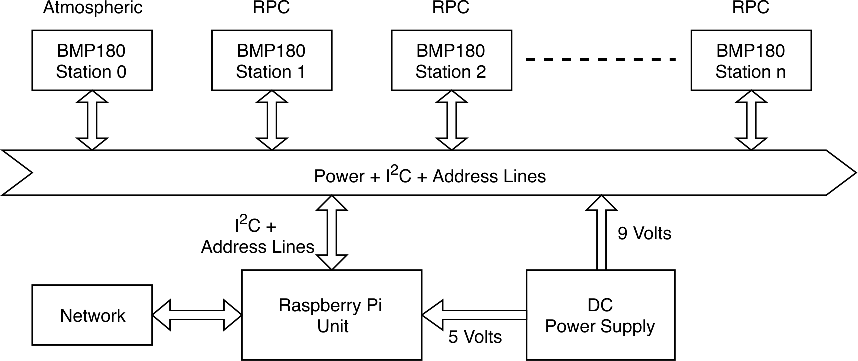
\includegraphics[width=0.9\textwidth]{leaktest_setup.pdf}
  \caption{Schematics of the `standalone' leak test setup.}
  \label{fig:schematics}
\end{figure}
In this setup, instead of measuring the differential pressure using the conventional manometer, the absolute pressure and temperature inside and outside of the gas gap are measured using the sensor module, BMP180 manufactured by BOSCH\cite{bmp180}. The BMP180 is a piezo-resistive sensor having an accuracy of 0.7\,mmWC and 0.05\,$^{\circ}$C in the measurement of pressure and temperature respectively. This sensor is capable of recording data samples for the minimum time interval of 76\,ms. The leak test module is shown in Figure~\ref{fig:setup}(\subref{fig:pc3}). 
\begin{figure}
  \centering
  \begin{subfigure}[b]{0.34\textwidth}
    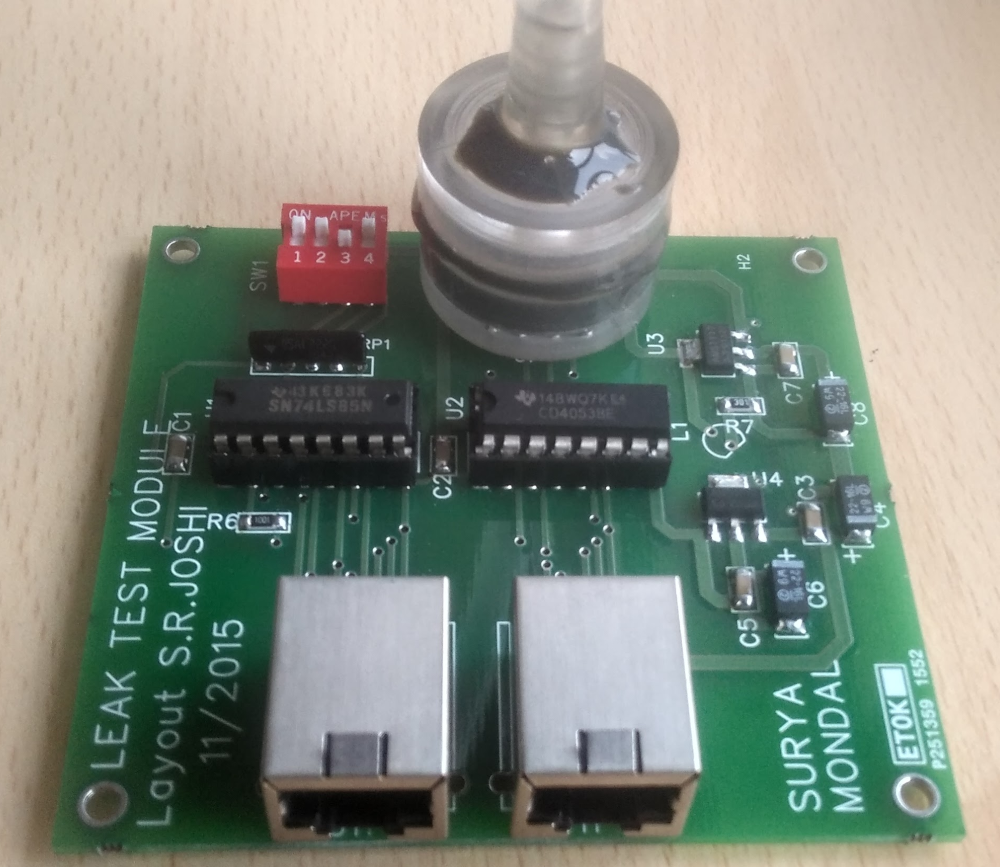
\includegraphics[width=\textwidth]{pc3.png}
    \caption{Leak Test Module.}
    \label{fig:pc3}
  \end{subfigure}
  \begin{subfigure}[b]{0.64\textwidth}
    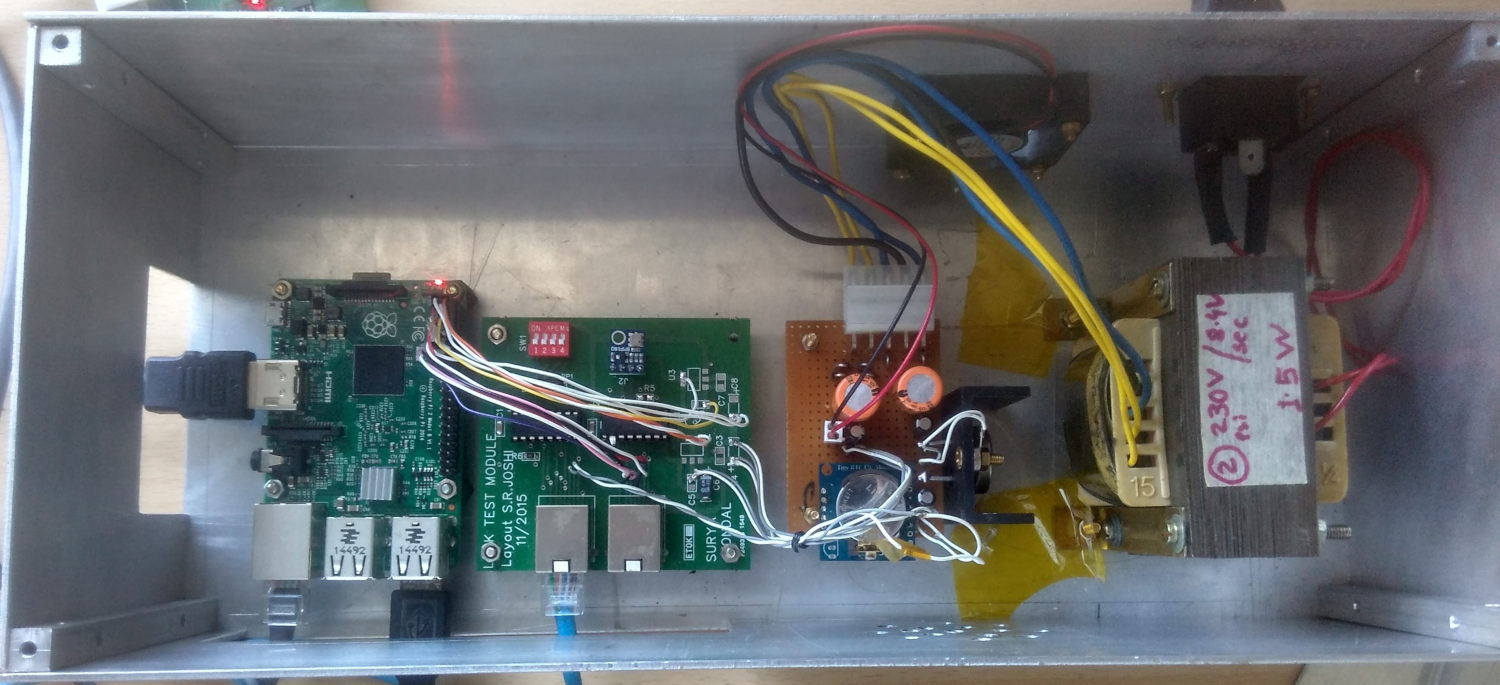
\includegraphics[width=\textwidth]{pc2.png}
    \caption{Raspberry Pi B \& Power Supply Module.}
    \label{fig:pc2}
  \end{subfigure}
  \caption{Leak Test Setup.}
  \label{fig:setup}
\end{figure}
Each of such modules will record the pressure and temperature for one gas gap. The pressure and temperature data recorded by the module is readout using a \textit{Raspberry Pi\,v2\,B} (Pi) unit\cite{rpi} shown in Figure~\ref{fig:setup}(\subref{fig:pc2}). The data is stored on the on-board memory of the Pi unit. As shown in Figure~\ref{fig:setup}(\subref{fig:pc3}), each module has two bus ports. This allows to daisy-chain several leak test modules and can be controlled from a single Pi unit.

The common bus mainly consists of Power, Data and Address lines. To avoid the voltage drop in the supply line over long distance, 9\,V DC is supplied from the Pi End and converted to required voltage at each test module. A 4-bit DIP switch is used on each module to set a unique address for itself. The Pi acquires the data from each station by selecting its unique address. So, only one test module is allowed to communicate with the control unit at a time. As 4-bit address lines are used in this setup, a maximum of fifteen gas gaps can be tested simultaneously. The system is scalable to handle more gas gaps simultaneously, by simply adding more address lines. One of the leak test module is dedicated to record the ambient pressure and temperature for the test duration.

The data from the BMP180s can also be acquired without wires by microcontrollers equipped with WiFi modules (i.e. NodeMCU module\cite{nodemcu2015}), eliminating the need of the wired common bus and Pi Unit. One of such setup is shown in Figure~\ref{fig:leakwifi}. 
\begin{figure}
  \centering
  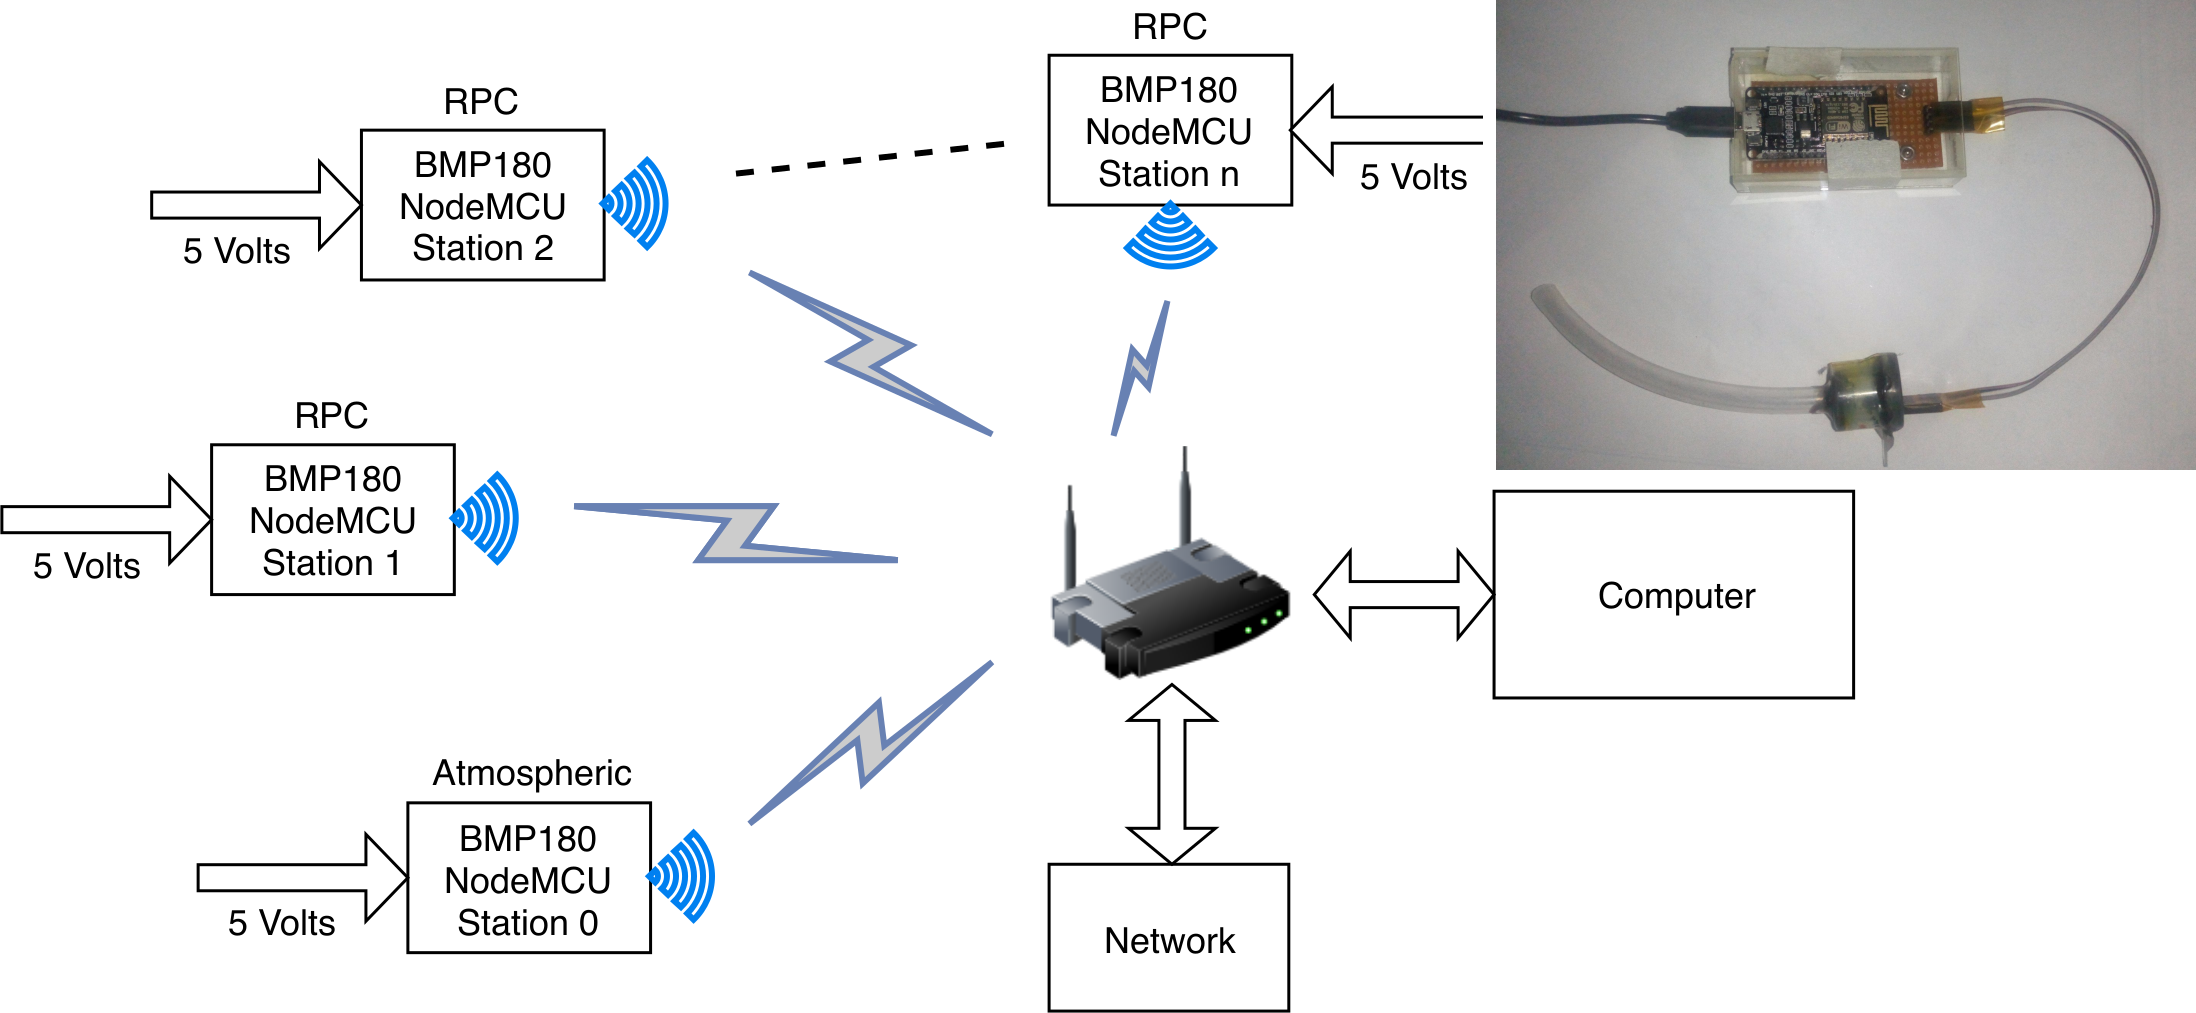
\includegraphics[width=0.99\textwidth]{leaktest_setup_wifi_all.png}
  \caption{Schematics of the WiFi-based leak test setup and one of the test-module (in the inset).}
  \label{fig:leakwifi}
\end{figure}
This setup requires an operational WiFi network at the premises to send the data to a computer on the same network. If the network is connected to the internet, then the data can be stored at any remote location also. The test-modules, being low-power devices, can also be powered with small power~banks which makes it hugely advantageous while being used at large warehouses. Also, the elimination of the long wires makes this setup immune to the electromagnetic interference from other sources. Though this setup is not `standalone', it is truely scalable which can handle any number of RPC gaps being tested without changing any of the basic designs elements.

In the current setup, the pressure and temperature data from each sensor along with the atmospheric pressure and temperature data are recorded continuously with a specified interval of $3$\,seconds. The final data recorded for a gas gap has the ambient pressure and temperature, the gas gap pressure and temperature and the time stamp for each measurement. Using these measurements, the method to quantify the leakage is discussed in the section~\ref{sec:calculation}.

\subsection{Detection of Button Pop-Ups}\label{sec:button}
The structural stability of the RPC is maintained by the polycarbonate buttons. However, it is observed that sometimes the glue which used to attach the buttons to the glass plates, fails to hold under pressure which results in detaching of the buttons from the glass plates.\footnote{Hereafter such an event is referred to as `button pop-up'.} This weakens the structure of RPC. Also during detector operations, this will increase the spacing between the glass plates, thus decreasing the effective electric field resulting in reduced signal strength. Also, for any working RPC, it is necessary that the glue used to attach the buttons to the glass plates continues to hold under pressure. For any RPC gas gap, even if only one button is not attached, that glass gap will not be suitable to hold more pressure as eventually the glue for more and more buttons will give away, making the gas gap weaker. Hence, it is essential to detect any `button pop-up' events during the leak test.

With each `button pop-up' event, the volume of RPC gap increases which in turn results in a decrease in the pressure inside the gap. Thus the pressure difference between the outside and inside of the gap decreases. In the plot of pressure difference with time, this effect will be observed as a sudden drop in the pressure difference. Figure~\ref{fig:button} shows the variation of pressure difference with time for a RPC where there are `button pop-up' events. 
\begin{figure}
  \centering
  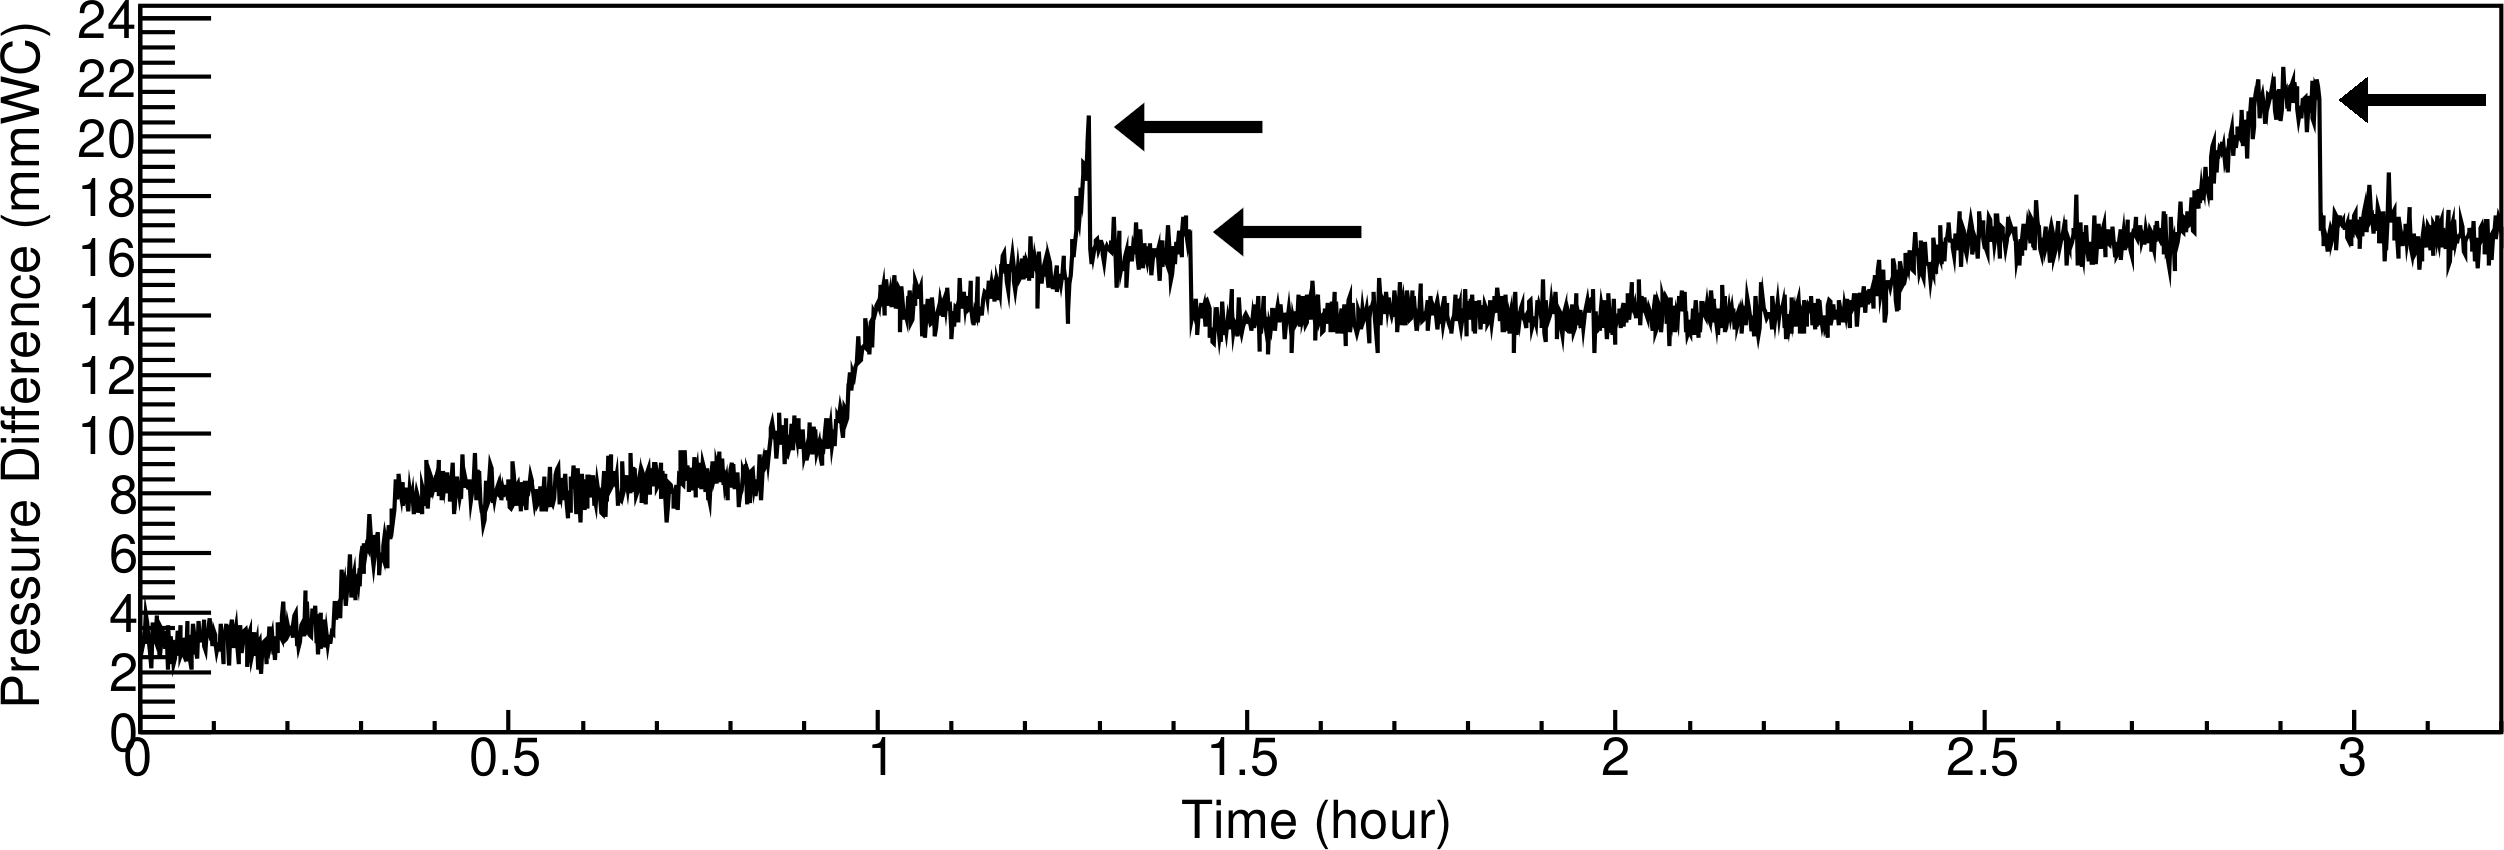
\includegraphics[width=0.99\textwidth]{button.png}
  \caption{Variation of pressure difference with time showing button pop-ups.}
  \label{fig:button}
\end{figure}
It can be observed in the figure that there are three `button pop-up' events (pointed by arrows) in this RPC. As seen here, these `button pop-up' events results in decrease of the pressure difference in a fraction of time. These events cannot be detected with conventional manometer unless the pressure is recorded continuously using a precise differential pressure sensor. Hence, the apparatus, described in the current paper, is very helpful in detecting the `button pop-up' events during the test.

It is also to be noted that the method to quantify the leakage discussed in the following, fails if the data includes button-pop event(s) in it.

\subsection{Leak Rate Calculation}\label{sec:calculation}
The variation of temperature of the gas gap and variation of pressure in the gas gap as well as atmosphere respectively with time are illustrated in Figure \ref{fig:temp}(a) and \ref{fig:temp}(b). 
\begin{figure}[h]
  \centering
  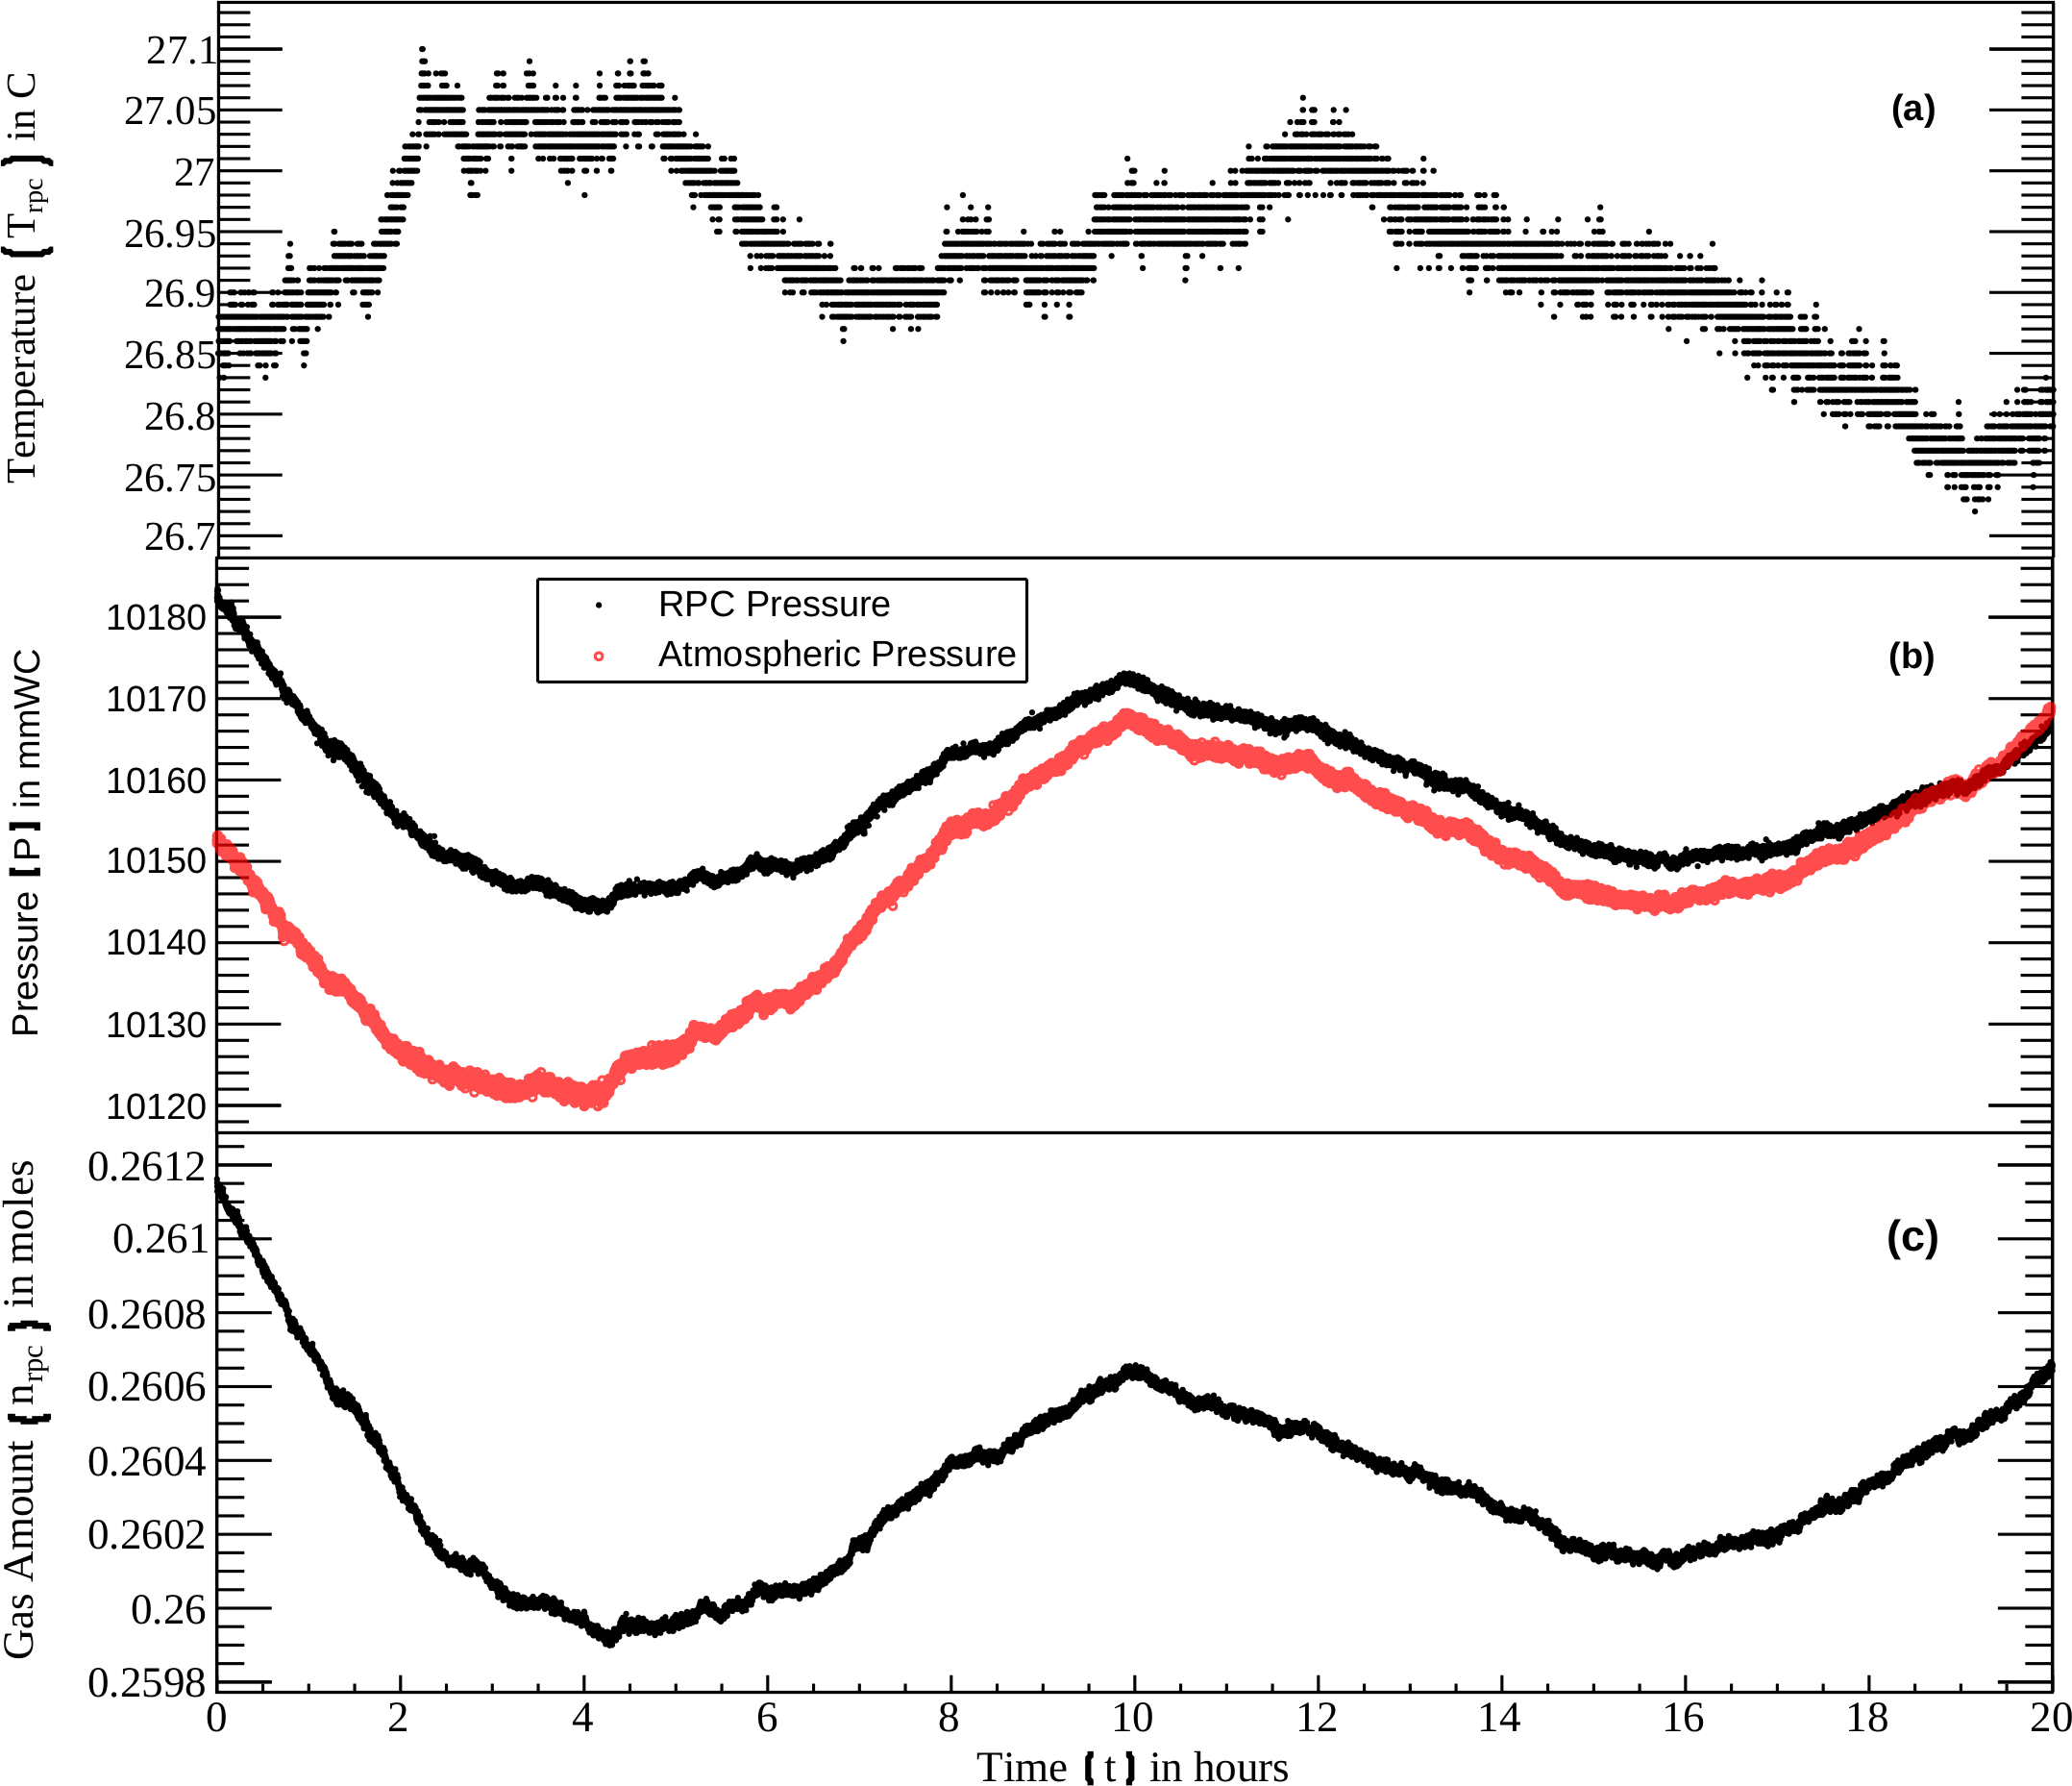
\includegraphics[width=0.99\textwidth]{all_57_gen.png}
  \caption{\textbf{(a)} Variation of temperature $\left(T_{\textrm{rpc}}\right)$ with time, \textbf{(b)} Variation of atmospheric $\left(P_{\textrm{atm}}\text{ : Black}\right)$ and RPC $\left(P_{\textrm{rpc}}\text{ : Red}\right)$ pressure with time, \textbf{(c)} Amount of gas in the RPC with time assuming $V_{\textrm{rpc}}=6.3$\,litres for sample RPC gap-1.}
  \label{fig:temp}
\end{figure}
The periodic variation of the atmospheric pressure shown in Figure~ \ref{fig:temp}(b) is called the Solar Atmospheric Tide. It can be observed that the pressure inside the gap is following the trend of atmospheric pressure. This implies that the volume of the gap changes with the change of atmospheric pressure. The change in room temperature also affects the pressure inside the RPC, again affecting the volume of the RPC gap. This change of the volume during the leak test poses the main difficulty in calculating the leak rate.

Now, from the Ideal Gas Law, the amount of gas ($n$), inside a chamber of volume $V$, can be calculated at time $t$ using the following equation,\footnote{All the values of $P$, $V$ and $T$ are converted suitably to calculate the value of $n$ in mole.}
\begin{equation}
  n_{\textrm{rpc}\mid t}=\frac{P_{\textrm{rpc}\mid t}V_{\textrm{rpc}\mid t}}{RT_{\textrm{rpc}\mid t}} \label{mole}
\end{equation}
where, $R$ is the ideal gas constant having the value 8.314\,J\,mole$^{-1}$\,K$^{-1}$. From the dimensions of the gas gap, the volume of the RPC is estimated to approximately 6.3\,litres. Taking this into consideration, the amount of gas inside the gap can be calculated using equation~\ref{mole}. The Figure~\ref{fig:temp}(c) shows the variation of the amount of gas within the gap with respect to time. The instantaneous leak rate of a gap can be quantified as the slope of this plot.

To estimate the absolute leak rate, the Poiseuille's equation for compressible fluids\cite{poiseuille} is used. The Poiseuille's equation of Leak Rate at time $t$ for compressible fluids is given in equation \ref{eq:poiseuille},
\begin{equation}
  \underbrace{\left.\frac{\mathrm{d}n_{\textrm{rpc}}}{\mathrm{d}t}\right| _t}_\text{flow/leak rate}=\underbrace{\textrm{C}_{\textrm{Leak}}}_\text{flow/leak constant}\times\underbrace{\left(\frac {P_{{\textrm{rpc}\mid t} }^{2}-P_{{\textrm{atm}\mid t} }^{2}}{2P_{{\textrm{rpc}\mid t} }}\right)}_\text{effective pressure difference}\label{eq:poiseuille}
\end{equation}
where, $\textrm{C}_{\textrm{Leak}}$ depends on the path of leakage (i.e. crack, hole, etc) and the viscosity of the gas mixture and it quantifies the leakage in the system.\footnote{The viscosity of the gas is assumed to be constant over the small changes of room temperature during the test period. In case of large changes in temperature, the changes in the value of viscosity are also needed to be considered.} The Figure~\ref{fig:preQt} shows the leak rate $\left(\frac{\mathrm{d}n_{\textrm{rpc}}}{\mathrm{d}t}\right)$ which is calculated from Figure~\ref{fig:temp}(c) as a function of the effective pressure difference $\left(\frac{P_{\textrm{rpc}}^{2}-P_{\textrm{atm}}^{2}}{2P_{\textrm{rpc}}}\right)$.\footnote{It is assumed that mole\,$\simeq$\,22.4\,litres for better visualisation.} 
\begin{figure}
  \centering
  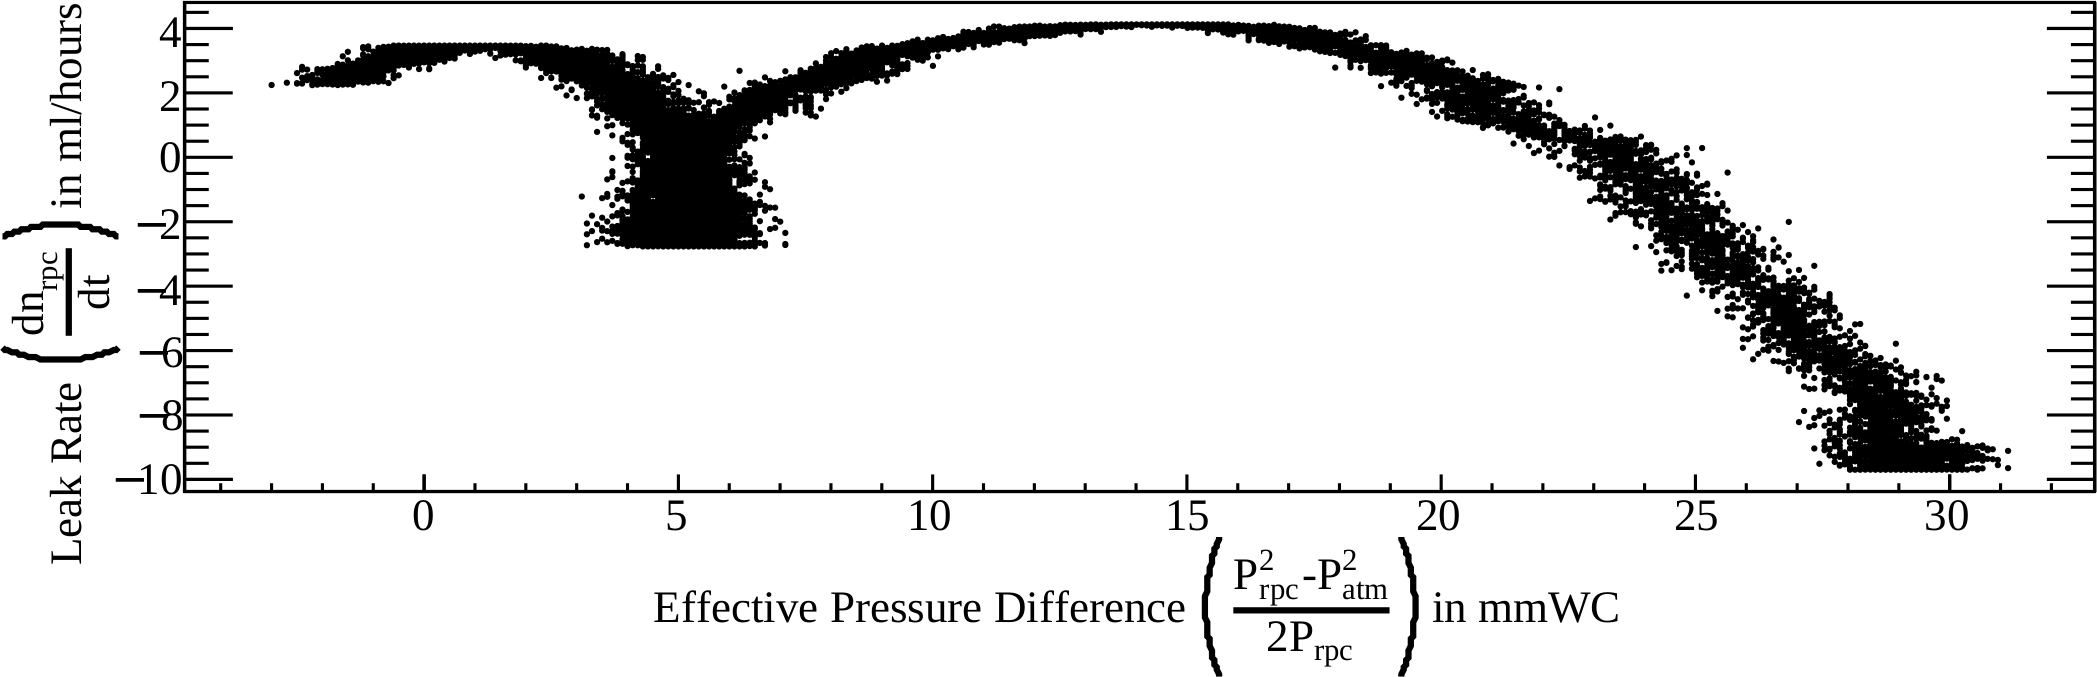
\includegraphics[width=0.99\textwidth]{Q_dP_57_pre.png}
  \caption{$\frac{\mathrm{d}n_{\textrm{rpc}}}{\mathrm{d}t}$ vs $\frac{P_{\textrm{rpc}}^{2}-P_{\textrm{atm}}^{2}}{2P_{\textrm{rpc}}}$ for the sample RPC gap-1 without any correction.}
  \label{fig:preQt}
\end{figure}

According to the equation~\ref{eq:poiseuille}, it is expected to behave as a straight line passing through the origin with the slope $\left(\textrm{C}_{\textrm{Leak}}\right)$ quantifying the leakage in the system but it can be clearly observed that it is not a straight line. Also, the gas gap under test is sealed from the inlet. Hence, no more gas is getting filled but the Figure~\ref{fig:temp}(c) shows an apparent increase in the amount of gas inside the gap. This discreapancy is appearing as the change in the volume of the RPC is not accounted in the calculation. Now, as the change in the volume of the RPC gap cannot be measured directly during the test period, a different approach is adopted.

To compensate this change in volume, the volume of the RPC gap at time $t$ is represented by the equation~\ref{vcterm},
\begin{equation}
  V_{\textrm{rpc}\mid t} = \underbrace{V_{\textrm{rpc}}}_{\text{Approx. Volume}}\times\underbrace{\left(1-x_T\left(T_{\textrm{rpc}\mid t}-T_{\textrm{rpc}\mid t=0}\right)\right)}_{\text{Correction for Temperature Change}}\times\underbrace{\left(1-x_P\left(P_{\textrm{atm}\mid t}-P_{\textrm{atm}\mid t=0}\right)\right)}_{\text{Correction for Pressure Change}}\label{vcterm}
\end{equation}
where, $T_{\textrm{rpc}\mid t=0}$ and $P_{\textrm{atm}\mid t=0}$ are equal to $T_{\textrm{rpc}}$ and $P_{\textrm{atm}}$ at time\,$t=0$, respectively.\footnote{Suffix `atm' denotes the measurements acquired from atmosphere.} Assuming that the change in volume is linear to both the atmospheric pressure and the room temperature, two independent linear correction terms ($x_P$ and $x_T$) are introduced.\footnote{Present method of estimation of leak cannot handle change in volume caused by `button pop-up' event during the period of leak test.} Using the equation~\ref{vcterm} in the equation~\ref{mole}, the $n_{\textrm{rpc}}$ is represented in the equation~\ref{eq:ct}.
\begin{equation}
  n_{\textrm{rpc}\mid t}=\left(\frac{V_{\textrm{rpc}}}{R}\right)\left(\frac{P_{\textrm{rpc}\mid t}}{T_{\textrm{rpc}\mid t}}\right)\left(1-x_T\left(T_{\textrm{rpc}\mid t}-T_{\textrm{rpc}\mid t=0}\right)\right)\left(1-x_P\left(P_{\textrm{atm}\mid t}-P_{\textrm{atm}\mid t=0}\right)\right) \label{eq:ct}
\end{equation}

Now, in order to calculate the $n_{\textrm{rpc}}$ for the test period using the equation~\ref{eq:ct}, it is required to find the suitable values for the correction factor, $x_P$ and $x_T$. The value of these correction factors are found (or minimised) against the plot in the Figure~\ref{fig:preQt}. The method to find the values is described bellow.
\begin{enumerate}[a.]
\item \label{itm:cor1} For a chosen combination of values of $x_T$ and $x_P$, $n_{\textrm{rpc}}$ is calculated using equation~\ref{eq:ct} and then is plotted against time.
\item The plot of $\frac{\mathrm{d}n_{\textrm{rpc}}}{\mathrm{d}t}$ vs $\frac{P_{\textrm{rpc}}^{2}-P_{\textrm{atm}}^{2}}{2P_{\textrm{rpc}}}$ is then prepared using the plot described in the process [\ref{itm:cor1}].
\item \label{itm:cor2} The plot of $\frac{\mathrm{d}n_{\textrm{rpc}}}{\mathrm{d}t}$ vs $\frac{P_{\textrm{rpc}}^{2}-P_{\textrm{atm}}^{2}}{2P_{\textrm{rpc}}}$ is then fitted with a straight line and $\chi^2/\textrm{ndf}$ is calculated.
\item \label{itm:cor3} The processes [\ref{itm:cor1}--\ref{itm:cor2}] are repeated for different combination of $x_T$ and $x_P$, and  $\chi^2/\textrm{ndf}$'s are obtained for each combinations. The $\chi^2/\textrm{ndf}$ values for each combination of $x_T$ and $x_P$ are shown in the Figure~\ref{fig:xp}. For a particular combination of $x_T$ and $x_P$, the $\chi^2/\textrm{ndf}$ will be minimum which is shown in the Figure~\ref{fig:xp}.
  \begin{figure}[h]
    \centering
    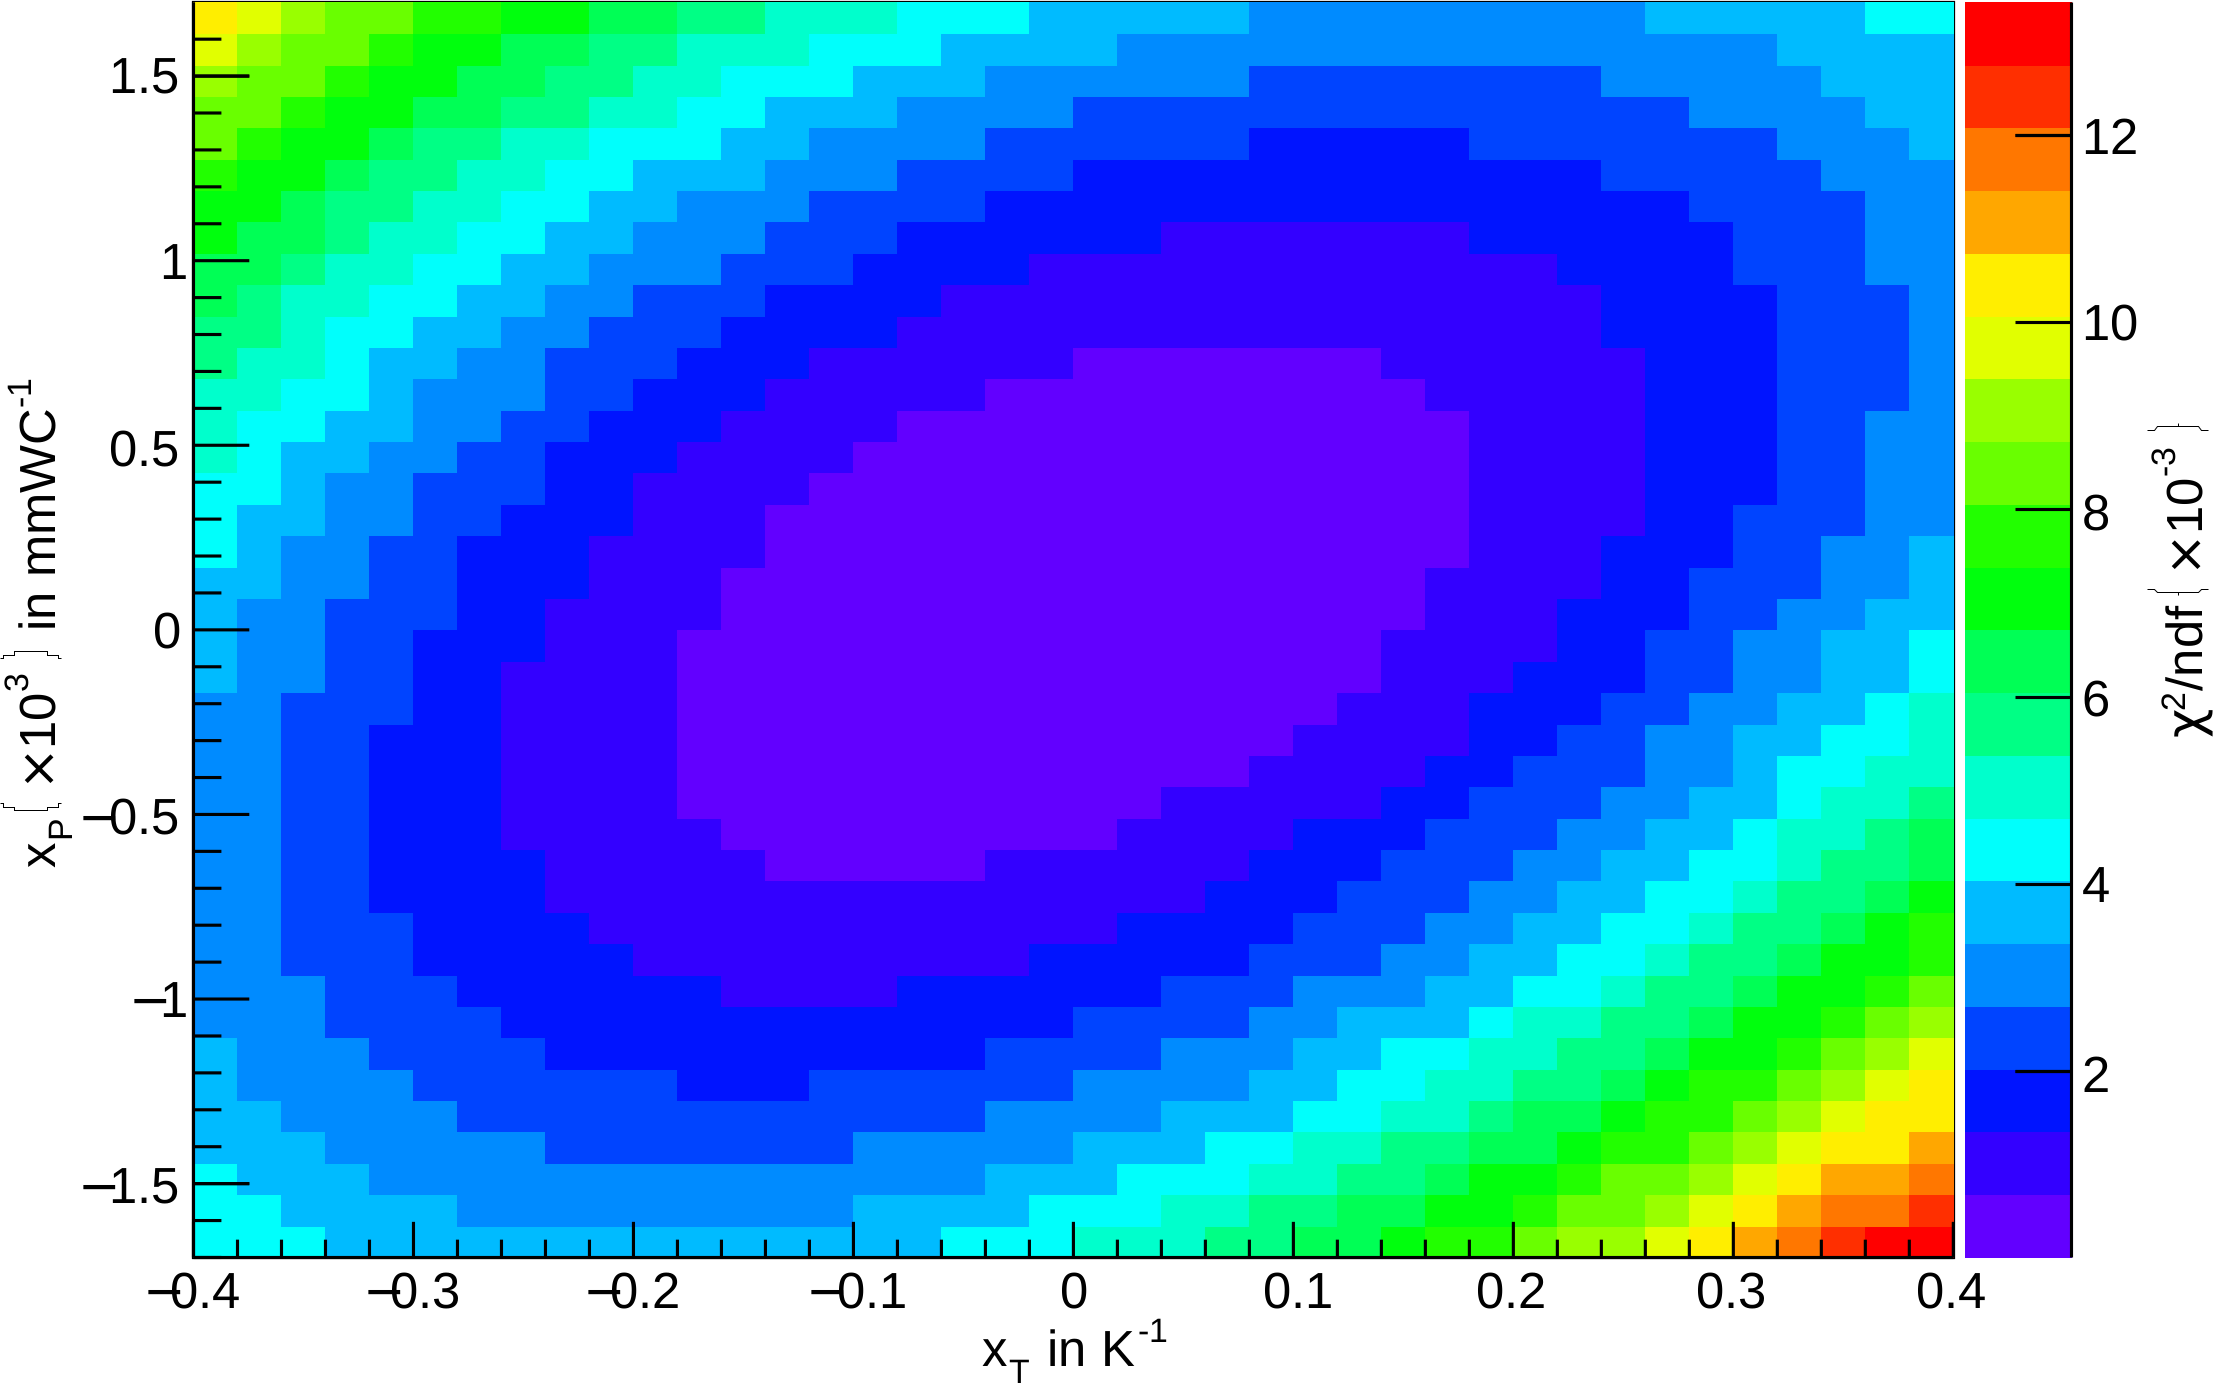
\includegraphics[width=0.8\textwidth]{cor_factors.png}
    \caption{$\chi^2/\textrm{ndf}$ values of the straight line fit for the plots of $\frac{\mathrm{d}n_{\textrm{rpc}}}{\mathrm{d}t}$ vs $\frac{P_{\textrm{rpc}}^{2}-P_{\textrm{atm}}^{2}}{2P_{\textrm{rpc}}}$ for different combinations of $x_T$ and $x_P$ for sample RPC gap-1.}
    \label{fig:xp}
  \end{figure}
\item  In order to reduce the uncertainties at the minimum $\chi^2/\textrm{ndf}$, the procedures [\ref{itm:cor1}--\ref{itm:cor3}] are repeated for multiple iterations with subsequently smaller range of $x_T$ and $x_P$ to obtain the final values. 
\end{enumerate}

 In the current case of sample RPC gap-1, the correction terms at minimum $\chi^2/\textrm{ndf}$ are found to be 
\[x_T=-3.23\times10^{-3}\textrm{\,K}^{-1}\textrm{ and }x_P=7.83\times10^{-5}\textrm{\,mmWC}^{-1}\textrm{.}\]

The negative value of the $x_T$ denotes that the volume of the gas-gap increases with increase in room temperature and the positive value of the $x_P$ denotes that the volume of the gap decreases with increase in atmosheric pressure. In both the cases, the values do not contradict with the Ideal Gas Law. After including the best-fit values of $x_T$ and $x_P$ in the equation~\ref{eq:ct}, the amount of gas inside the RPC gap $\left(n_{\textrm{rpc}}\right)$ against time is shown in the Figure~\ref{fig:with}.
\begin{figure}[h]
  \centering
  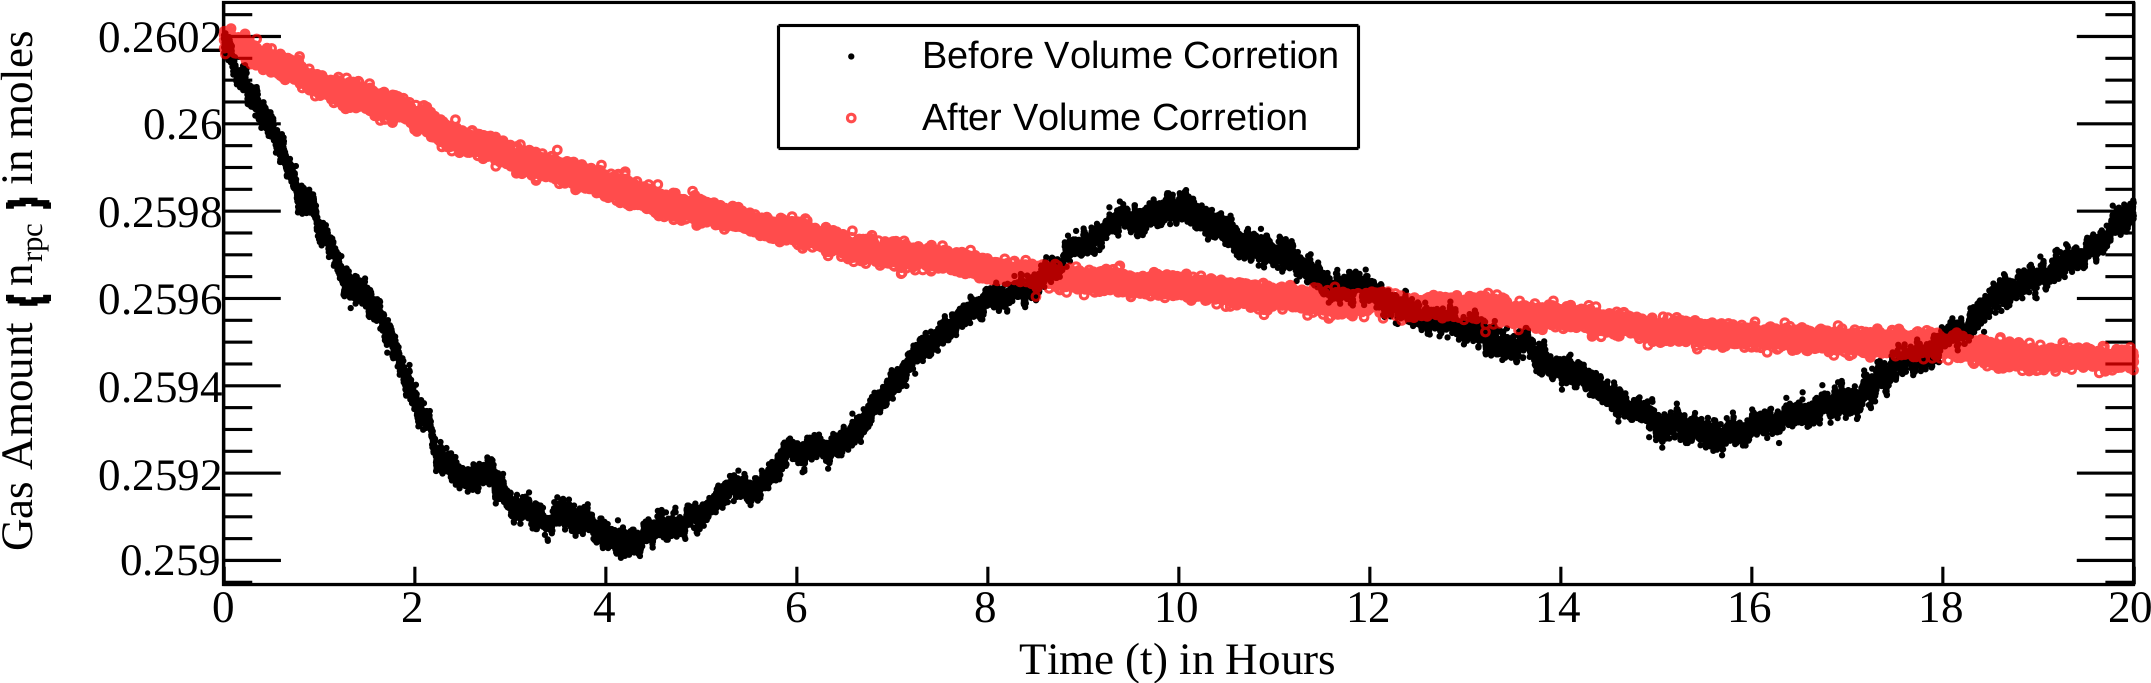
\includegraphics[width=0.99\textwidth]{M_t_57.png}
  \caption{Amount of gas in the RPC before (Black) and after (Red) correction for sample RPC gap-1.
  }
  \label{fig:with}
\end{figure} 
It can been noted in the Figure~\ref{fig:with} that the apparent increase of gas amount seen earlier without the correction is resolved after applying the volume correction. The effect of the volume currection also can be observed in the plot of $\frac{\mathrm{d}n_{\textrm{rpc}}}{\mathrm{d}t}$ vs $\frac{P_{\textrm{rpc}}^{2}-P_{\textrm{atm}}^{2}}{2P_{\textrm{rpc}}}$ in the Figure~\ref{fig:qt} which follows a nice straight line as expected from the Poiseuille's equation.
\begin{figure}[h]
  \centering
  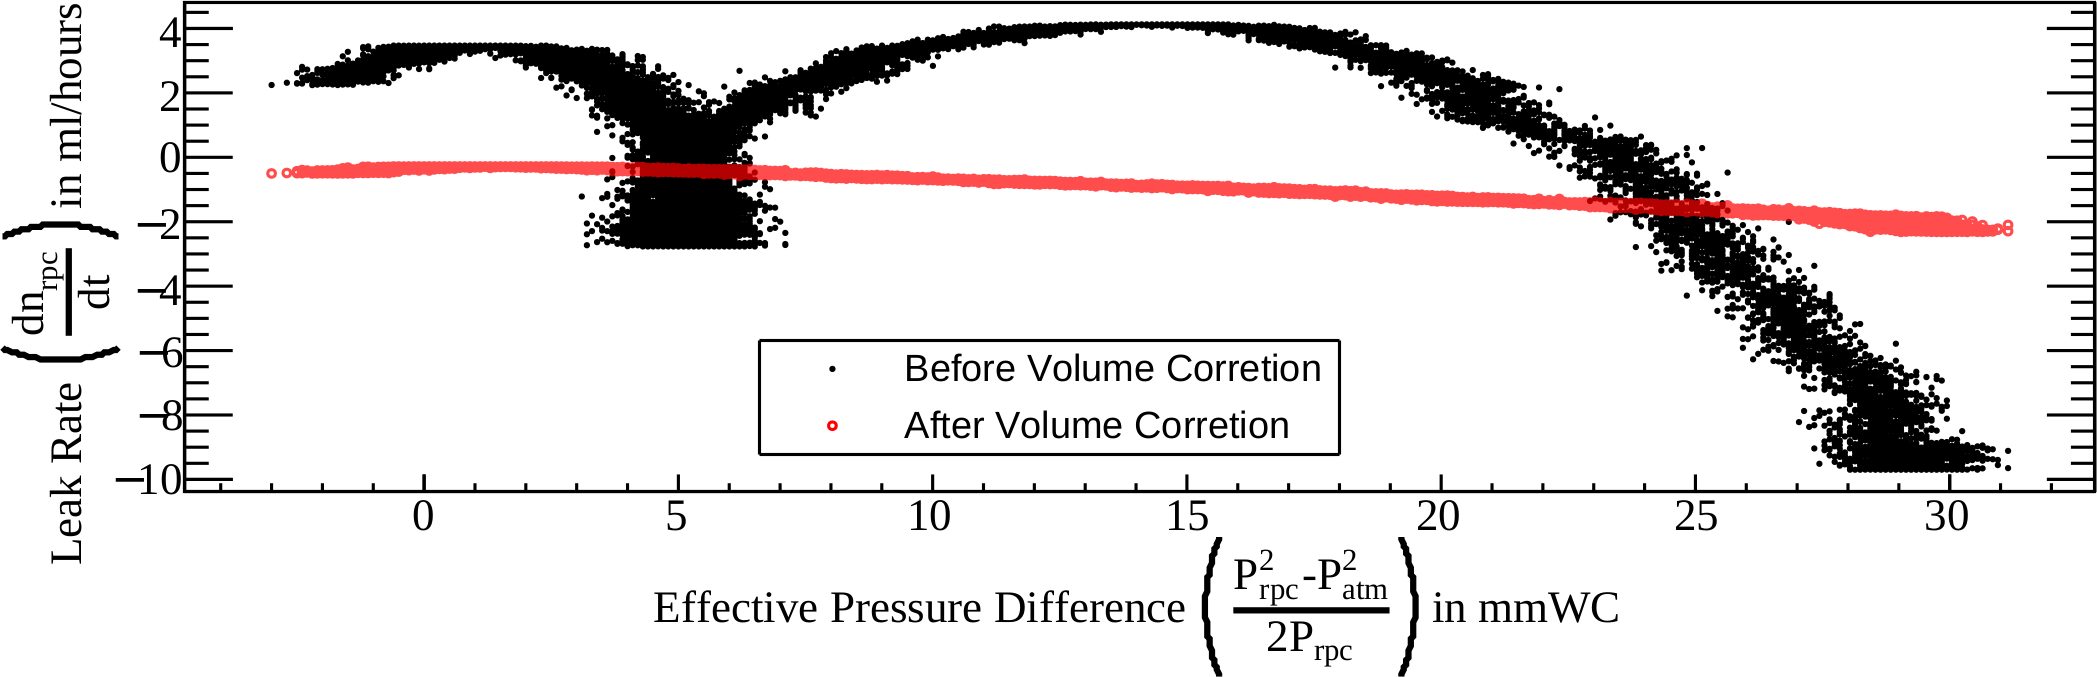
\includegraphics[width=0.99\textwidth]{Q_dP_57.png}
  \caption{$\frac{\mathrm{d}n_{\textrm{rpc}}}{\mathrm{d}t}$ vs $\frac{P_{\textrm{rpc}}^{2}-P_{\textrm{atm}}^{2}}{2P_{\textrm{rpc}}}$ plots before (Black) and after (Red) correction for sample RPC gap-1.}
  \label{fig:qt}
\end{figure}

The value of $\textrm{C}_{\textrm{Leak}}$ calculated from the Figure~\ref{fig:qt} is
\[\textrm{C}_{\textrm{Leak}}=-\left(6.73\pm 0.007\left(\textrm{stat}\right)\right)\times 10^{-2}\textrm{\,ml\,hour$^{-1}$\,mmWC$^{-1}$}.\]

The negative value of $\textrm{C}_{\textrm{Leak}}$ implies that the leakage of gas is from inside to outside, which again agrees with the value of the pressure difference. Now, if the this RPC gap is kept under a constant pressure difference of 20\,mmWC, then it would leak a total of 1.442\,$m$mol or 32.3\,ml gas in 24\,hours. This RPC gap thus can be tagged as leaky.

Figure~\ref{fig:with1} and \ref{fig:qt1} show the test results for another RPC gap (namely, gap-2).
\begin{figure}
  \centering
  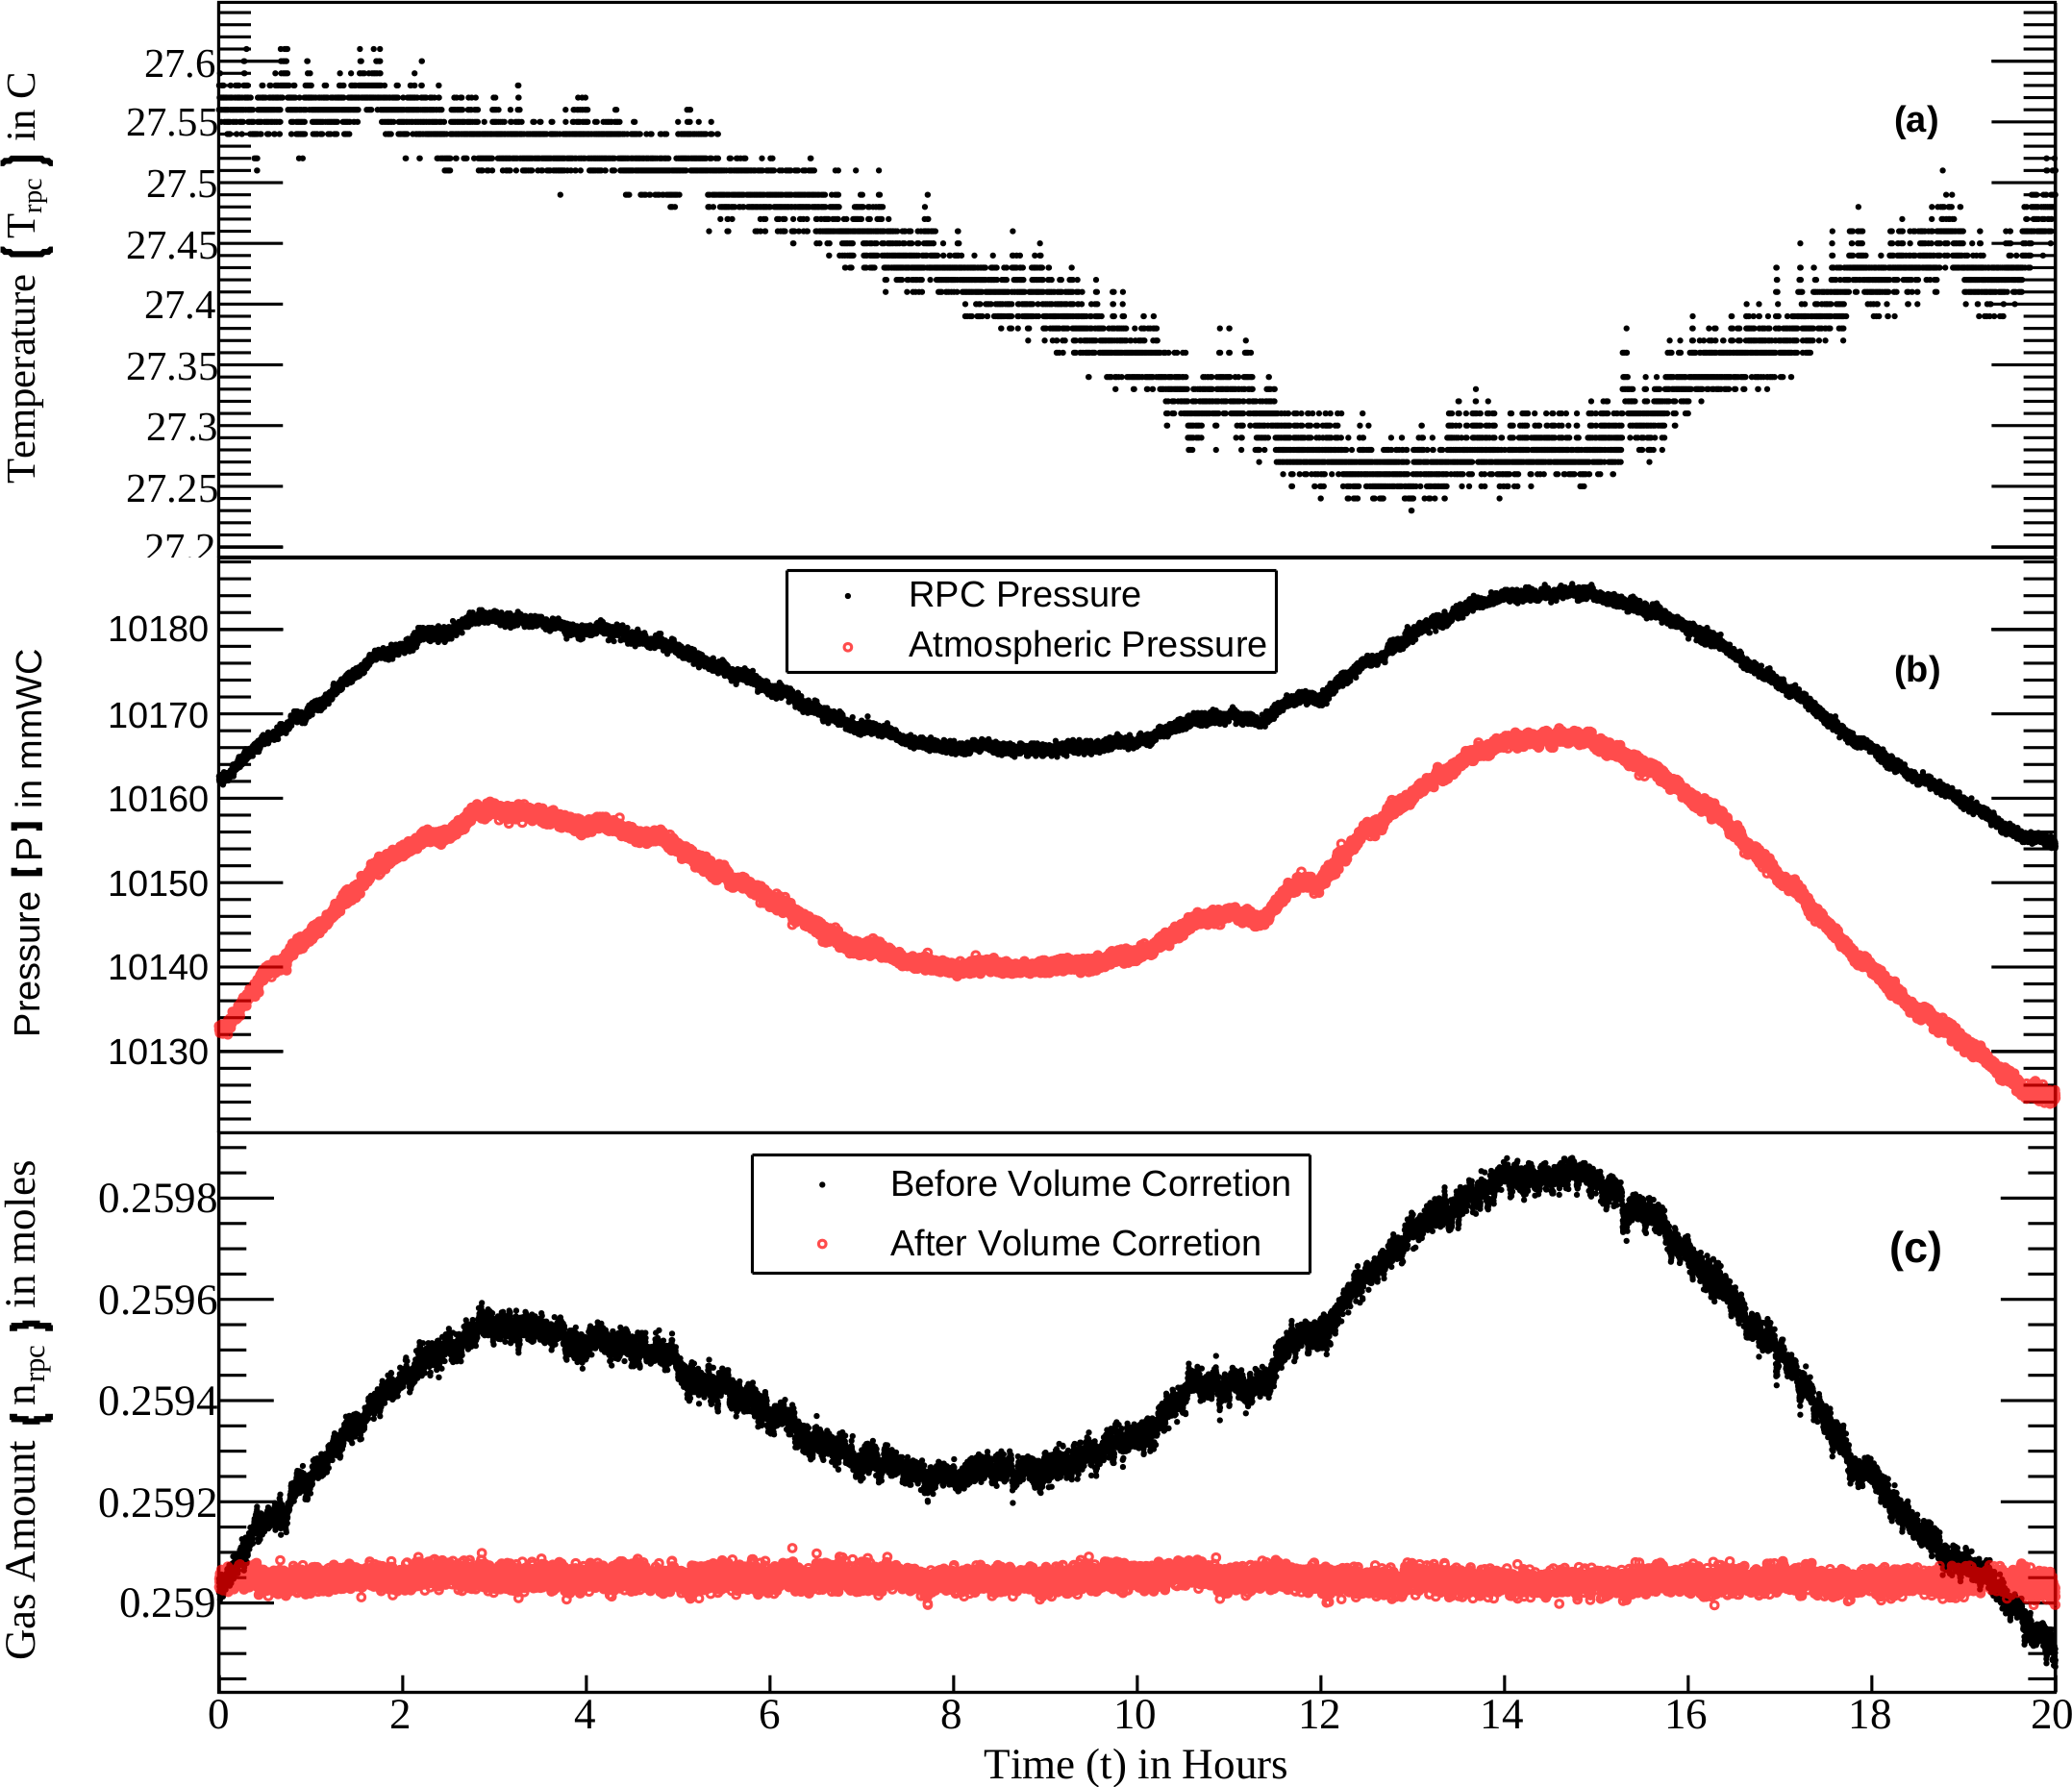
\includegraphics[width=0.99\textwidth]{all_130_gen.png}
  \caption{\textbf{(a)} Variation of temperature ($T_{\textrm{rpc}}$) with time, \textbf{(b)} Variation of atmospheric ($P_{\textrm{atm}}$ : Black) and RPC ($P_{\textrm{rpc}}$ : Red) pressure with time, \textbf{(c)} Amount of gas in the RPC before (Black) and after (Red) correction for sample RPC gap-2.}
  \label{fig:with1}
\end{figure}
\begin{figure}
  \centering
  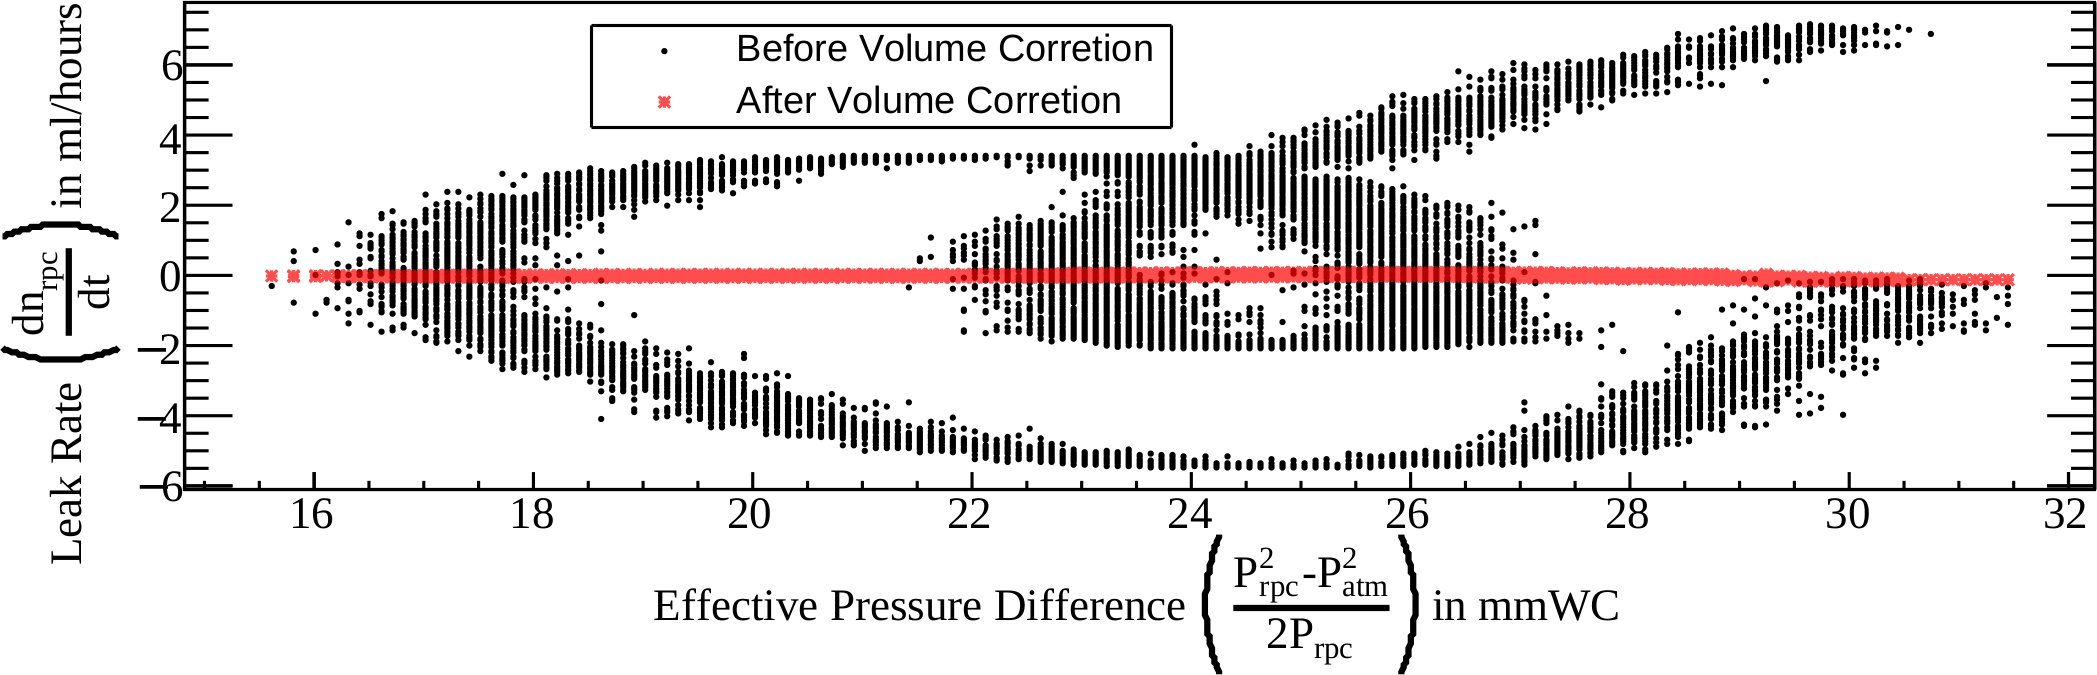
\includegraphics[width=0.99\textwidth]{Q_dP_130.png}
  \caption{$\frac{\mathrm{d}n_{\textrm{rpc}}}{\mathrm{d}t}$ vs $\frac{P_{\textrm{rpc}}^{2}-P_{\textrm{atm}}^{2}}{2P_{\textrm{rpc}}}$ plots before (Black) and after (Red) correction for sample RPC gap-2.}
  \label{fig:qt1}
\end{figure}
From Figure~\ref{fig:qt1}, the value of $\textrm{C}_{\textrm{Leak}}$ for this RPC gap is estimated to be
\[\textrm{C}_{\textrm{Leak}}=-\left(5.1\pm 0.15\left(\textrm{stat}\right)\right)\times 10^{-4}\textrm{\,ml\,hour$^{-1}$\,mmWC$^{-1}$}.\]
In this case, the total leak would be 10.93\,$\mu$mol or 0.245\,ml of gas within 24\,hours if a constant pressure difference of 20\,mmWC is maintained. The leak from this RPC gap is thus very small.

One of the aim of this study is to estimate the optimum (or minimum) time required for calculating the leak rate satisfactorily. As seen in the Figure~\ref{fig:temp}, the duration of the test is about 20\,hours. Several calculations of the leak rate $\left(\textrm{C}_{\textrm{Leak}}\right)$ are performed starting with the same data set but up-to different lengths. In the Figure~\ref{fig:time}, the value of $\textrm{C}_{\textrm{Leak}}$ for different duration of data is plotted.
\begin{figure}
  \centering
  \includegraphics[width=0.99\textwidth]{conf_57.png}
  \vspace*{10pt}
  \includegraphics[width=0.99\textwidth]{conf_130.png}
  \caption{Leak rate estimation for data sets of different length for (a) RPC gap-1 and (b) RPC gap-2.}
  \label{fig:time}
\end{figure}
For RPC gap-1, it can be observed that a minimum of 7-8 hours is required to estimate the leakage without significant uncertainty. This method requires a significant amount of data to fit the $\frac{\mathrm{d}n_{\textrm{rpc}}}{\mathrm{d}t}$ vs $\frac{P_{\textrm{rpc}}^{2}-P_{\textrm{atm}}^{2}}{2P_{\textrm{rpc}}}$ plots in order to get proper results. Hence, the minimal time required for a test will depend on the quantity of the leakage and also the environmental conditions during the test. If the leak rate is very small then more time is needed. In the case of RPC gap-2, it can be observed from Figure~\ref{fig:time}(b) that about 7 hours is required to estimate leak rate with an uncertainty of $\sim 2\times 10^{-3}$\,ml\,hour$^{-1}$\,mmWC$^{-1}$, but about 15 hours is needed to have a result with uncertainty less than $\sim 2\times 10^{-4}$\,ml\,hour$^{-1}$\,mmWC$^{-1}$.

